\documentclass[conference]{IEEEtran}
\IEEEoverridecommandlockouts
% The preceding line is only needed to identify funding in the first footnote. If that is unneeded, please comment it out.
\usepackage{cite}
\usepackage{hyperref}
\usepackage{amsmath,amssymb,amsfonts}
\usepackage{algorithmic}
\usepackage{graphicx}
\usepackage{subfig}
\usepackage{booktabs}
\usepackage{tablefootnote}
\usepackage{textcomp}
\usepackage{xcolor}
\usepackage{array}
\def\BibTeX{{\rm B\kern-.05em{\sc i\kern-.025em b}\kern-.08em
T\kern-.1667em\lower.7ex\hbox{E}\kern-.125emX}}
\newcolumntype{P}[1]{>{\centering\arraybackslash}p{#1}}
\newcolumntype{M}[1]{>{\centering\arraybackslash}m{#1}}
\begin{document}

\title{The Influence of Clarity on Career Choice and Academic Success in First Year\\
}

\author{\IEEEauthorblockN{Mohammed Gathoo}
\IEEEauthorblockA{\textit{School of Computer Science} \\ \textit{and Applied Mathematics} \\
\textit{University of the Witwatersrand}\\
Johannesburg, South Africa \\
migathoo@outlook.com}
\and
\IEEEauthorblockN{Shalini Dukhan}
\IEEEauthorblockA{\textit{School of Animal, Plant} \\ \textit{and Environmental Sciences} \\
\textit{University of the Witwatersrand}\\
Johannesburg, South Africa \\
shalini.dukhan@wits.ac.za}
\and
\IEEEauthorblockN{Ritesh Ajoodha}
\IEEEauthorblockA{\textit{School of Computer Science} \\ \textit{and Applied Mathematics} \\
\textit{University of the Witwatersrand}\\
Johannesburg, South Africa \\
ritesh.ajoodha@wits.ac.za}
}

\maketitle

\begin{abstract}
According to the statistics gathered from the Council of Higher Education (CHE), an observation has been made that an increase in the rate of admissions to science degrees do not have a corresponding increase in the rate of graduates from said degrees. Much research on this phenomenon has been conducted in order to find the underlying causes of this observation, including examination of family and peer influence, roles of schools and educators and an individual's affinity towards science. This research aims to make use of machine learning techniques to build a system that can determine which aspects of a student's life most influences their performance by looking at their Science Identity, background factors and schooling experience, as well as predict their success (determining whether a student has passed or failed). The results produced will be of a binary classification type, indicating whether a student has passed of failed based on potential aspects of influence outlined by previous research. These results produced intend to substantiate the use of a combination of statistical and computational methods such as machine as effective, reliable and robust means of predicting student success at a first-year university level for a biological science degree.
\end{abstract}

\begin{IEEEkeywords}
Biology degrees, Machine learning, Student Identity
\end{IEEEkeywords}

\section{Introduction}
Research has shown the student retention and throughput in the Science faculty at a South African university is not increasing at the rate at which the number of students who are admitted into science-related courses are increasing (according to statistics produced by the CHE at \url{https://www.che.ac.za/publications/vital-stats}). There are various influences at play within a student’s life that contributes towards the academic success of a student (see \cite{b1} and \cite{b2}). These include patterns with regards to career path knowledge and the decisions made thereof, relative interest in the work they are studying, and external factors related to a student’s personal life such as culture, religion, gender, and social class.

While there is an abundance of research done with regards to this topic from various angles, this study aims to look at this problem through the lens of Science Identity, including the factors contributing to its development and the extent to which it influences the success of a student's performance in university.

This study aims to answer the following question: To what extent do students who are certain of their choice for a job in science perform better in first year compared to students who are unsure of their career path? Answering this question will hopefully provide insight into the reason the number of students who graduate with a degree in Biological Sciences are fewer than the number of those who enter first year. This could potentially enable further insight into how a multitude of factors could influence student performance in biological sciences, the formation of science identity and provide an understanding into how career guidance might be able to mitigate the attrition that is currently taking place during undergraduate years in biology.

This research aims to look at how factors such as familial support, peer roles, schooling background and university experiences, as well as their knowledge on biology related careers affects the development of a Science Identity (see \cite{b3}), as well as to see the extent at which each of these influences affects the performance of a student. This research seeks to use a Bayesian Network, a probabilistic model which represent the conditional dependency of random variables as a graphical model, combined with machine learning algorithms such as Bayesian estimation and maximum likelihood estimation to perform factor analysis in the model.

This study will make use of a dataset containing information gathered from a survey done on 130 First Year biology students in 2019, modelled using a Bayesian Network. In total, six different models will be used to predict student success, and the performance of each model will be compared with each other. Analysis of each model will be carried out in order to determine which of the features provided greatest influence the outcome of a student's academic success of their first year in a biological science degree. Student Profiles will be used as a base for training and testing, consisting of influences that affect Student Identity outlined by Science Identity.

This research hopes to provide a robust system that is capable of analysing a student's background and aspects of their Science Identity and predicting their academic university success, contributing to our understanding of the problem and providing a potentially new way of seeking solutions to mitigate the low graduation rate observed.

\section{Related Work}

This sections provides a literature review that presents research already done regarding the topic, such as identity formation, Science Identity and developed prediction models. This will provide a baseline understanding of the topic, as well as gain insight into what has already been contributed to the body of knowledge regarding this topic, specifically that which is relevant to this research.

\subsection{Identity Formation}

Research has been done to conceptualize the idea of one's identity. One particular journal \cite{b4} does so by conceptualizing the idea of a personal identity and collective identity and its formation, and then viewing the influence it has on a person’s motivated action and behavioural choices, beginning by outlining a social cognitive model elaborated to evaluate social and motivational factors that influence achievements and behaviours such as career aspirations.

The social cognitive theory model (acquiring knowledge directly related to observations) used by Jacquelynne Eccles \cite{b4} allows for making of certain predictions with regards to the behaviour of an individual based on their personal and collective identity and the formation thereof. This leads to the belief that motivated behavioural choices are related to motivational aspects of identity. It is evident the choices an individual makes and the relative value these decisions have is influenced by many factors that play in the development of one’s science identity. 

It also goes on to argue that identities comprise of three components: a value component encompassing the importance and attractiveness a person attaches to the group of characteristics one is a member of; a content component which includes the beliefs a person has about which tasks, activities, goals, etc. are associated with successful action; and an expectancy component that details the person's belief in whether or not they are capable of carrying out these tasks, activities, goals, etc. These three components are said to interact with each other over the lifetime of the individual, interacting with one another over a wide range of experiences which ultimately influences behavioural choices. The writer also outlines the way in which various identities and beliefs influence development, specifically making use of gender as an example and outlining how these identities specifically affect women and girls in their choices and motivations in educational settings with respect to educational decisions.

\subsection{Science Identity}

The concept of Science Identity and its development appears to be of great contribution towards a student's success in science related fields, not just at university level but also at a schooling level. Science identity is the sense of who students are, what they believe they are capable of, and what they want to do and become in regard to science \cite{b5} . A study was done \cite{b6} delving deep into its development during university and using it as a predictor of success with regards to science-related careers. The results of this study show a correlation between the value of science identity prior to and during university (high value usually results in increased importance of its exploration), as well as the importance of science identity stability and how compromising its well-being (e.g. consistently receiving a bad grade in science) may negatively influence and destabilize science identity. The study conducted intended to answer multiple research questions, the one of relevance to my project being whether science identity trajectories could predict science career outcomes after university. The study began by gathering data from participants during first year and continued annually until graduation.

The analysis conducted on the gathered data involved fitting growth mixture models using descriptive statistics and examining the resulting trajectory plots. Results showed that differential trajectories predicted the pursuit of science related careers, and the students who were characterized as having a high or moderate science identity continued to identify as such with little or no change. The study also showed, however, that university was a period of potentially volatile change in a student's identity if they experienced initially low science identity. Studies have shown that science identity was a strong predictor of student’s choices and greatly increases my understanding of factors influencing and supporting students’ trajectories towards careers in science \cite{b7}.

In a study done to investigate science identity during university \cite{b8}, three latent classes were identified, labelled \textit{High with Transitory Incline} reflecting high science identity involving slight increases and decreases throughout 4 years of college, \textit{Moderate-High and Stable} reflecting high science identity with non-noticeable change over the 4-year degree, and \textit{Moderate-Low and Early Decline} reflecting a relatively low science identity in the first year, followed by a decrease in the remainder of the 4-year degree. The study found a clear distinction in trajectories of science identity in students regarding the latent classes, trajectories related to career outcomes, fist-year competence and responsibility, gender and race/ethnicity. The study highlights a potential need for science identity development before college, as well as supporting and maintaining high science identity over the period of the 4-year degree. Declines in science identity throughout college that results displayed amongst minority students could be mitigated by support provided by academic institutions either during first year or prior to college in order to improve their belief in their ability to develop and/or maintain high science identity. The study contributes the understanding that becoming a scientist is more involved and nuanced than obtaining skills and knowledge for success, but also having developed and maintained a belief that they are capable of being a scientist and achieving their goals.

Factors outside of the educational space also contribute greatly to the development of science identity. A study conducted to gauge a student’s interest in science \cite{b9} enables observation of the way in which gender, social class and ethnicity influences and contributes towards a young learner's attitude towards science. Surveys found that learners might possess a positive attitude towards science, but display a lack of interest in 'the idea of being a scientist'. This highlights the lack of supporting a broader perception of science and scientists amongst primary school students by educators and researchers amongst others. Gender, ethnicity and social class were shown to have minor influence overall, suggesting improving aspirations in science directed at specific groups may be less beneficial compared to targeted improvement taking into account wider ranges of characteristics and attitudes. After interviewing a number of students as well as their parents', research found that while positive attitudes towards science are not translating into aspirations in science, a positive foundation for venturing into science is present. 17\% of respondents agreed with the idea of being a scientist, while 29\% displayed interest in a 'job using science'. This leaves us with the question of what the best age for educational intervention is, and how best to engage students with the work pertaining to science, among many others. The research conducted does not convey the proportion of students who could potentially develop a stronger, more positive attitude towards science after primary school.

\subsection{Data Mining and Prediction Models}

The use of machine learning techniques is not foreign to prediction of student success. Many have been employed to examine other aspects of a student’s success. Some have taken to examining the high school performance of students and using various predictive models to determine success and comparing it to the APS (Admission Points Score) and its correlation to student success \cite{b10}. Important factors and attributes were selected according to the Tinto (1975) framework, one which groups characteristics into 3 groups: \textit{Background, Individual} and \textit{Pre-College/Schooling}. Models such as Naive Bayes, Logistic Regression and Multilayer Perceptrons (among others) were used, the lowest being a Multilayer Perceptron having a prediction accuracy of 67.74\% while the model with the highest prediction accuracy, 69.18\% proved to be the Naive Bayes Model.

Others have used machine learning techniques to investigate biographical observations such as socioeconomic factors that determine student success and psycho-social factors that affect student performance to see the role they play in a student’s success, not just at a particular year, but during each year of a 3-year degree, using models such as C4.5 Decision Tress, Random Forests and Sequential Minimal Optimization to predict student performance in advance \cite{b11}. In this study, Random Forests model proved to have the highest predictive accuracy at each year of study, with at least 93\% accuracy. 

As shown, there are a multitude of algorithms that can be used to predict student success, each with their own advantages and disadvantages. Their use will allow for the bench-marking of performance to compare with other techniques used in the development of this system.

\section{Methodology}

This research aims to create a system that can examine Science Identity, background factors and schooling experience in order to predict the success or failure of a student in a biology science degree. This section discusses the data being used and how it was engineered to fit its intended way of use, the models that were implemented, and the results thereof.

\subsection{Data}
The dataset used for this study is a synthetic dataset generated through the use of a Bayesian Network with a known ground truth distribution. The original data was taken from surveying 129 first-year students between the ages of 18 and 21. Categorical encoding of nominal and ordinal data was carried out for ease of use and compatibility with the models being used.

Several features consisted of the 4-point Likert scale rating as possible answers, one that allows a person to express their agreement or disagreement with a particular statement (1 = Strongly Agree, 2 = Agree, 3 = Disagree, 4 = Strongly Disagree).

Due to the confidential nature of the data being used, Ethics Clearance had to be obtained through the WITS University Human Research Ethics Committee (Non-Medical). Protocol Number CSAM-2002-06W is proof of clearance provided with the help of chairperson Dr Helen Sarah Robertson.

\subsection{Pre-processing and Feature Engineering}
The features in this dataset covers 8 aspects of a student's life: General Biographical Data, Family support and Background, School Background and Experience, Peer Role, Self Reflection and Grades.

Feature categories such as General Biographical Data, Family Support and School Experience have a wide variety of answers and, therefore, make use of integer encoding. Other feature categories such as Family and School background, Peer Role and Self Reflection are rated according to the Likert scale, also using integer encoding for each level of the 4-point scale.

The target variable is the final outcome of a student, i.e. whether they have passed or not, which is inferred from a feature in the dataset. Said target variable contains 2 possible values, \textit{Passed} (a student obtained an end-of-year mark 50\% or higher) or \textit{Failed} (a student obtained an end-of-year mark lower than 50\%).

Lastly, the data was balanced by using over-sampling due to few students with having done the survey with features such as School Experience having multiple entries per student.

\subsection{Models}
In this study, six machine learning predictive models were used for the prediction of the target variable: Na\text{\"i}ve Bayes Classifier, Generalized Linear Model, Deep Neural Network (DNN), Multilayer Perceptron (MLP), Random Forests, and Sequential Minimal Optimization (SMO).

The DNN and MLP are similar in implementation with regards to sharing the underlying structure of a neural network (input/output and hidden layers, activation functions, weights and biases), but differ in the number and size of hidden layers, therefore affecting the training times of the respective models. The DNN will make use of the ReLU (Rectified Linear Unit) activation function,
\begin{equation}
R(z)=max\{0,z\}
\end{equation}
and the MLP will make use of the sigmoid activation,
\begin{equation}
F(z)=\frac{1}{1+e^{-z}}
\end{equation}
where \(z\) is the sum of the product of each input \(x_i\) and their weight \(w_i\) for \(i \in \{0,...,n\}\) (\(z=\sum{_{i=1}^n}{x_i w_i}\)).

\subsection{Evaluation, Performance and Accuracy}

\subsubsection{Evaluation and Validation}
Model effectiveness will be evaluated using the \textit{k}-fold cross-validation procedure, a re-sampling procedure used to evaluate machine learning models, It does so by splitting the data randomly into training and testing partitions, and then further partitioning the training dataset into \textit{k} folds (partitions) where \textit{k}-1 folds are used to train the model while the remaining \textit{k}-th fold is used for validation. This process is repeated until all folds have been used at least once for validation. 10 folds will be used for this study.

\subsubsection{Performance}
Confusion matrices are a useful tool for the visualization of classification algorithm performance. Given that the target variable has two distinct classes, the confusion matrix will have dimensions \(2 \times 2\) as depicted in the table below.

\begin{table}
\caption{Confusion Matrix Structure}
\begin{center}
\begin{tabular}{c|c|c} 
\hline
& \textbf{Predicted Passed (+)} & \textbf{Predicted Failed (-)} \\ 
\hline
\textbf{Actual Passed (+)} & TP & FN \\ 
\hline
\textbf{Actual Failed (-)} & FP & TN \\
\hline
\end{tabular}
\begin{itemize}
Structure of confusion matrix where:
\item{True Positive: positive outcome predicted and it’s true}
\item{True Negative: negative outcome predicted and it’s true}
\item{False Positive: positive outcome predicted and it’s false}
\item{False Negative: negative outcome predicted and it’s false}
\end{itemize} and + and - denote positive and negative classes respectively.
\end{center}
\end{table}

\subsubsection{Accuracy}
The confusion matrix allows us to extract important metrics regarding the performance of our models, particularly \textit{Precision} (total positive outcomes), \textit{Recall} (total correctly predicted outcomes from positive class), and \textit{Accuracy} (total correct predictions).
\begin{equation}
Precision=\frac{TP}{TP+FP}
\end{equation}
\begin{equation}
Recall=\frac{TP}{TP+FN}
\end{equation}
\begin{equation}
Accuracy=\frac{TP+TN}{TP+TN+FP+FN}
\end{equation}

Using the results of Precision and Recall, we can also calculate another metric known as F-measure (or F-score), a measure the accuracy of the test factoring in Precision and Recall into a single score. F-measure is calculated as follows:
\begin{equation}
F-measure=\frac{2 \times Recall \times Precision}{Recall+Precision}
\end{equation}

\section{Results}

\subsection{Model Accuracies}
Table II shows the prediction accuracy of each of the six models implemented, as calculated according to equation (5).

\begin{table}
\caption{Model Accuracy Of Target Variable Prediction}
\begin{center}
\begin{tabular}{|c|c|} 
\hline
\textbf{Model Name} & \textbf{Accuracy \&} \\ 
\hline
Na\text{\"i}ve Bayes & 86.23 \\ 
\hline
Deep Neural Network & 84.49 \\
\hline
Generalized Linear Model & 82.82 \\
\hline
Multilayer Perceptron & 82.02 \\
\hline
Sequential Minimal Optimization & 81.47 \\
\hline
Random Forests & 80.55 \\
\hline
\end{tabular}
\caption*{\footnotesize Prediction accuracy of each implemented model calculated after 10-fold cross validation according to equation (5)}
\end{center}
\end{table}

Using 10-fold cross validation as means to validate the accuracy of the models, it is evident that, according to Table II, all models implemented were able to achieve an accuracy of at least 80\% with Random Forests having an accuracy of 80.52\%. The model with the highest accuracy was Na\text{\"i}ve Bayes, obtaining an accuracy of 86.21\%.

\subsection{Prediction Outcomes}
The dataset had an 0.8/0.2 split for training data and testing data. The confusion matrices in Figure 1 represent the prediction outcome of the models after having been tested on a dataset of just under 1500 data points.
\begin{center}
\begin{figure}
\centering
\subfloat[\centering Na\text{\"i}ve Bayes]{{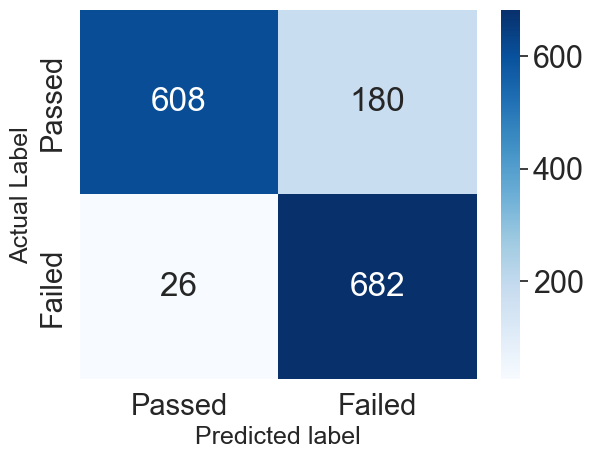
\includegraphics[width=3.5cm]{bnCF.png} }}%
\qquad
\subfloat[\centering Deep Neural Network]{{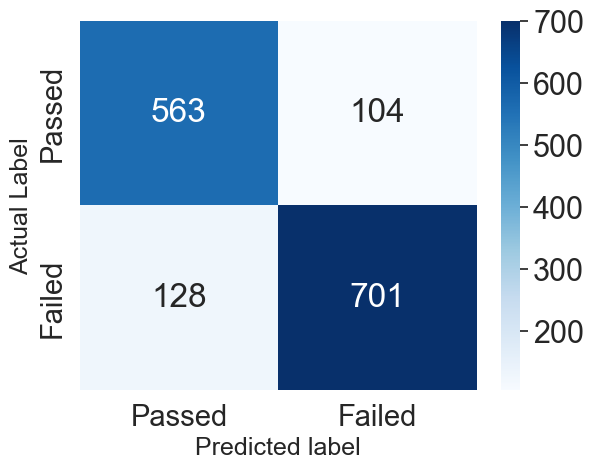
\includegraphics[width=3.5cm]{dnnCF.png} }}%
\qquad \\
\subfloat[\centering Generalized Linear Model]{{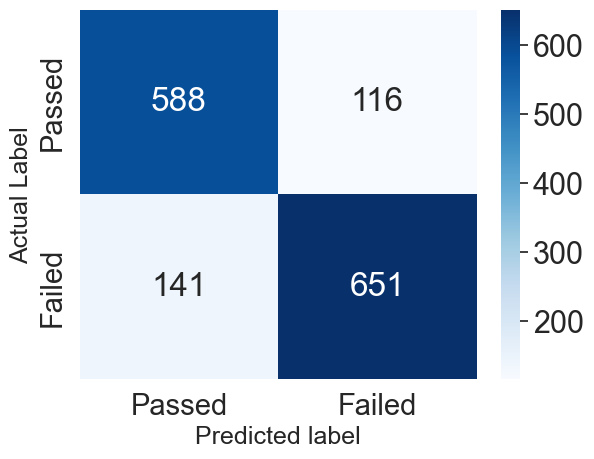
\includegraphics[width=3.5cm]{glmCF.png} }}%
\qquad
\subfloat[\centering Multilayer Perceptron]{{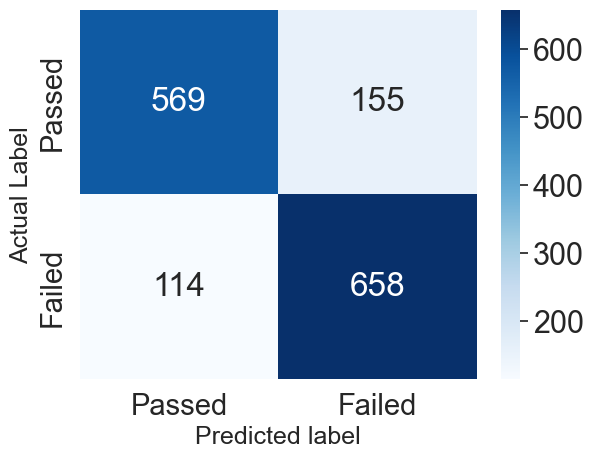
\includegraphics[width=3.5cm]{mlpCF.png} }}%
\qquad \\
\subfloat[\centering Sequential Minimal Optimization]{{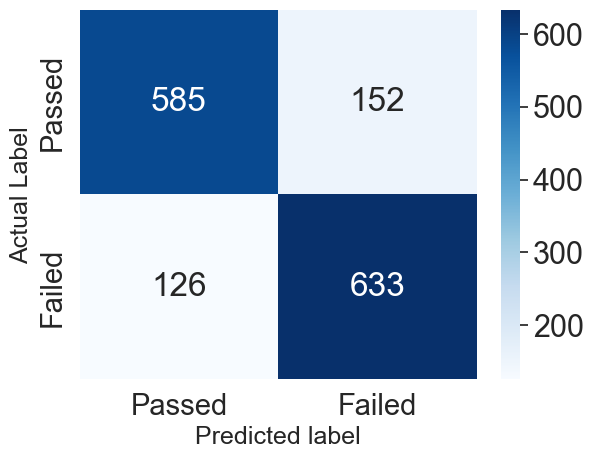
\includegraphics[width=3.5cm]{smoCF.png} }}%
\qquad
\subfloat[\centering Random Forests]{{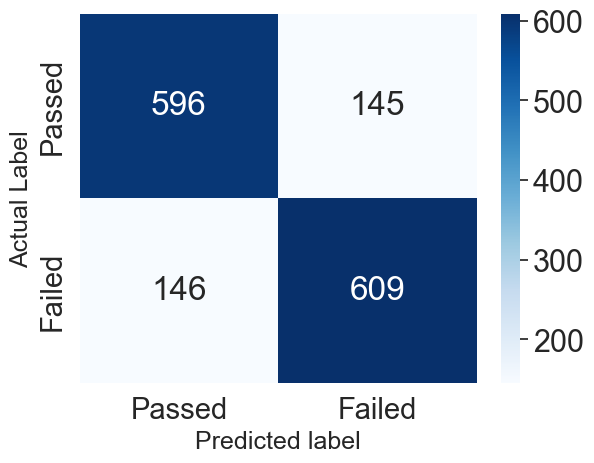
\includegraphics[width=3.5cm]{rfCF.png} }}%
\qquad \\
\caption{Confusion Matrices Depicting Model Prediction Outcomes on a Test Dataset of 1469 Data Points}%
\label{fig:example}
\end{figure}
\end{center}

Given the confusion matrices in Figure 1, we can calculate the Precision, Recall and F-measure for each model using equations (3), (4) and (6) respectively.
\begin{itemize}
\item{\textit{Na\text{\"i}ve Bayes}: this model achieved a Precision score of 0.96 and a Recall score of 0.84, resulting in an F-measure of 0.896.}
\item{\textit{Deep Neural Network}: this achieved a Precision score of 0.82 and a Recall score of 0.84, resulting in an F-measure of 0.840.}
\item{\textit{Generalized Linear Model}: this model obtained a Precision score of 0.81 and a Recall score of 0.84, resulting in an F-measure of 0.823.}
\item{\textit{Multilayer Perceptron}: this model obtained a Precision score of 0.83 and a Precision score of 0.79, resulting in an F-measure of 0.809.}
\item{\textit{Sequential Minimal Optimization}: this model attained a Precision score of 0.82 and a Recall score of 0.79, resulting in an F-measure of 0.804}
\item{\textit{Random Forests}: this model attained a Precision score of 0.80 and a Recall score of 0.80, resulting in an F-measure of 0.802}
\end{itemize}

Thus, it is evident that the F-measure score for all models correlate with the accuracy shown in Table II, all managing an F-measure over 0.8 for all six models. Na\text{\"i}ve Bayes' exceptional performance could be explained due to the naive conditional dependence assumption of the features being used, while the poorer performance of Random Forests (in comparison to the performance of other models) can be explained by the model potentially favouring suboptimal variables as a result of artificially biased predictor variables \cite{b12}.

\subsection{Feature Importance}
Having presented the performance of each model implemented using various metrics, next is the importance of each feature in the prediction of the target variable. Feature importance is measured using "permutation accuracy importance", calculated by the permutation of a predictor variable \(X_j\) while leaving the remaining predictor variables unpermutated, and predicting new a response \(\hat{Y}\). The measure for the predictor variable's importance will, therefore, be the difference in prediction accuracy before and after permutating \(X_j\).

\begin{table}
\caption{Feature Importance}
\begin{center}
\fontsize{10}{9}\selectfont
\resizebox{\columnwidth}{!}{%
\renewcommand{\arraystretch}{2.5}
\begin{tabular}{|M{5cm}|M{5cm}|}%
\hline
\textbf{Feature} & \textbf{Importance} \\ 
\hline
People in my family are interested in science & 0.154557 \\ 
\hline
My family is interested in the science course that I take & 0.131367 \\
\hline
My friends do not like science & 0.070677 \\
\hline
I do not enjoy visiting science museums and science centres & 0.057664 \\
\hline
My family has encouraged me to study science & 0.048199 \\
\hline
Level of support from your family from your studies this year & 0.041990 \\
\hline
Study/Learning approach used at university & 0.031062 \\
\hline
I prefer science class than visiting museums and centres & 0.030580 \\
\hline
My friends view science as nerdy & 0.024443 \\
\hline
My friends do not like to view science programs on tv & 0.020101 \\
\hline
My science teachers were enthusiastic about science & 0.019831 \\
\hline
My science teachers made science interesting & 0.017685 \\
\hline
My teachers encouraged me to do my best & 0.015634 \\
\hline
Visiting science museums and exhibits makes me want to learn more about the science topic & 0.014831 \\
\hline
My science teachers encouraged me to learn more about science & 0.013615 \\
\hline
My family is enthusiastic about a science career for me & 0.011686 \\
\hline
\end{tabular}%
}
\caption*{\footnotesize Feature Importance Determined using Permutation Accuracy (see \cite{b12}).}
\end{center}
\end{table}

Table III shows the importance of the features used in the dataset, however, there are 3 key things to make note of: 1. The table describes the 16 most important features with an importance \(>\) 0.01. Features less than were omitted from the table; 2. Feature importance was calculated after data processing and feature engineering, meaning some fields that were deemed unimportant were left out of the calculation; and 3. Some features had direct follow-up features that were meant to elaborate some of the data provided, these were not mentioned in Table III as well.

\section{Discussion and Limitations}
The experiments presented above demonstrates the use of machine learning techniques to predict the success of a student based on factors of their life that could influence their performance in university during a first year biology degree.

Six models were implemented and made use of a synthetic dataset for the task of prediction. After 10-fold cross validation, all six models were successful in achieving a minimum accuracy of 80\% as calculated according to equation (5). The Na\text{\"i}ve Bayes model proved to be the most accurate of all six implemented models, obtaining an accuracy 1.84\% higher than the second most accurate model, the Deep Neural Network. The weakest performing model was found to be the Random Forests model, having an accuracy measure 5.78\% less than the Na\text{\"i}ve Bayes model accuracy.

Revisiting the confusion matrices, some observations to note is that True Negative classes were predicted more often than True Positive classes. Na\text{\"i}ve Bayes showed to have a more varied difference between false predictions, predicting far more false negatives than false positives, overall predicting more negative labels for the dataset. This could be due to an artificial bias skewing the results, favouring some features over others. The rest of the models showed to have a more even distribution of false label predictions.

Having mentioned the similarities between the Multilayer Perceptron and the Deep Neural Network, their performance shows to be rather similar, with the Deep Neural Network having a higher accuracy due to a deeper structural implementation (more hidden layers with more nodes per layer). As mentioned previously, the MLP made use of the sigmoid activation function, the DNN made use of the ReLU (Rectifier Linear Units) activation function. While the DNN obtained a higher accuracy, it had taken a longer time to train as a result of its deeper structure, resulting in a trade-off between training time and prediction accuracy, despite ReLU activation function having shorter convergence time compared to the sigmoid activation function.

The importance of each feature representing some aspect of a student's life was determined using a Random Forests permutated accuracy importance to measure the importance of each feature in the prediction of the target variable. Table III shows that aspects regarding family and peer attitudes towards science proved to be of great influence on a student's performance, specifically interest in science as well as support for the student's pursuit of science. Educational figures such as teachers proved to be of less importance by comparison, as well as personal initiative to take part in science related activities.

Although we have achieved a high accuracy rate, there still exists limitations that hold back the potential of this study. Synthetic data does not always accurately represent real world events and observation, making it difficult to replicate them in theoretical scenarios. This may lead to the skewing of results obtained and, as a result, the employment of these models in the real world.

\section{Conclusion and Future Work}
The low rate at which students admitted into biology science degrees are completing their degrees, let alone finding careers have led to an abundance of research seeking to find a reason behind this observation. There is an abundance of research dedicated to this topic done in many different schools of thought and knowledge, from psychological to mathematical.

This research aimed at taking a more statistical and computational approach to finding an explanation for the low graduation rates by making use of several machine learning models to build upon the research already contributed to the topic, and examining various aspects of a student's life outlined by previous research with hopes of finding a potential way of preventing the low graduation rates.

The overall contribution of this research is to provide a more technical explanation for the observations we see today, with the hopes of identifying the key areas in the development of Science Identity as a possible major contributor and influential factor in student academic success during first year biology degrees. Identifying these key areas, as well as the circumstances of these areas can allow for the development of potential solutions to the problems being faced, helping mitigate the ramifications of students who are ill equipped to succeed academically, let alone at a high level.

Future work in this area may include the prediction of student grades given the dependent factors, more than just a binary classification problem. It may also include the facilitation of multiple entries per feature in a single data point for increased accuracy. Other solutions could be to implement more rigorous, robust models for prediction to mitigate error produced and obtain higher accuracies. This work may prove to be beneficial and can be extended to degrees beyond just those of biology, and even including other faculties.

\begin{thebibliography}{00}
\bibitem{b1} Eisenberg D, Downs MF, Golberstein E, Zivin K. Stigma and help seeking for mental health among college students. Med Care Res Rev. 2009 Oct;66(5):522-41. Epub 2009 May 19.
\bibitem{b2} Zajacova A, Hummer RA. Gender differences in education effects on all-cause mortality for white and black adults in the United States. Soc Sci Med. 2009 Aug;69(4):529-37. Epub 2009 Jul 7.
\bibitem{b3} Chen, S., Binning, K. R., Manke, K. J., Brady, S. T., McGreevy, E. M., Betancur, L., Limeri, L. B., and Kaufmann, N. (2021). Am I a Science Person? A Strong Science Identity Bolsters Minority Students’ Sense of Belonging and Performance in College. Personality and Social Psychology Bulletin, 47(4), 593–606.
\bibitem{b4} J. Eccles, "Who am i and what am i going to do with my life? personal and collective identities as motivators of action," Educational Psychologist,
vol. 44, no. 2, pp. 78-89, 2009.
\bibitem{b5} N. Brickhouse. ''Embodying Science: A Feminist Perspective on Learning. Journal of Research in Science Teaching.''2001. no. 38. pp 282 - 295.
\bibitem{b6} Robinson KA, Perez T, Nuttall AK, Roseth CJ, Linnenbrink-Garcia L. From science student to scientist: Predictors and outcomes of heterogeneous science identity trajectories in college. Dev Psychol. 2018;54(10):1977-1992.
\bibitem{b7} K. Robinson, T. Perez, A. Nuttall, C. Roseth, and L.-G. L., "From science student to scientist: Predictors and outcomes of heterogeneous science identity trajectories in college," Developmental Psychology, vol. 54, pp. 1977-1992, 2018.
\bibitem{b8} J. DeWitt, J. Osborne, L. Archer, D. Dillon, B. Willis, and B. Wong, "Young children's aspirations in science: The unequivocal, the uncertain and the unthinkable," International Journal of Science Education, vol. 2011, no. 6, pp. 1037-1063, 2013.
\bibitem{b9} Vincent-Ruz P, Schunn CD. The nature of science identity and its role as the driver of student choices. Int J STEM Educ. 2018;5(1):48. 
\bibitem{b10} T. Abed, R. Ajoodha and A. Jadhav, "A Prediction Model to Improve Student Placement at a South African Higher Education Institution," 2020 International SAUPEC/RobMech/PRASA Conference, 2020, pp. 1-6.
\bibitem{b11} N. Ndou, R. Ajoodha and A. Jadhav, "Educational Data-mining to Determine Student Success at Higher Education Institutions," 2020 2nd International Multidisciplinary Information Technology and Engineering Conference (IMITEC), 2020, pp. 1-8.
\bibitem{b12} Strobl C, Boulesteix AL, Zeileis A, Hothorn T. Bias in random forest variable importance measures: illustrations, sources and a solution. BMC Bioinformatics. 2007;8:25. Published 2007 Jan 25.
\end{thebibliography}

\end{document}